\documentclass[../main.tex]{subfiles}
\begin{document}
%\chapter{Results}\label{ch:O}
\section{The problem set}
For this work, we deal with 8-spin and 12-spin 2-SAT problems. The first set had 91 unique problems, while the second set had 1000 such problems. These problems were numbered from 1-1000 in case of the 12-spin problems, and 1-91 in case of the 8-spin problems. All the problems had a predetermined unique ground state, a highly degenerate first excited state, and only one avoided crossing between the ground and the first excited states. All the 8-spin problems had 9 pair-wise couplings, while the 12-spin problems had 13 such couplings. The success probability is then obtained by calculating the overlap between the known ground state and the state resulting from the code performing product evolution. Furthermore, for determining the energy spectra for specific problems, exact diagonalization method was employed.

For every problem belonging to the two sets, three annealing times are chosen to calculate the success probability. These correspond to $T_A \in \{ 10,100,1000 \}$. This chapter focusses on the results obtained for the original Ising Hamiltonian, i.e. in the absence of any triggers. All the results corresponding to the problems of the 8-spin set are shown in the appendix.

\section{Second-order Suzuki-Trotter Product formula algorithm}
Since the Suzuki-Trotter product-formula algorithm is an approximation to solve the TDSE, the numerical error $\lvert \lvert U(t)-\tilde{U}_2(m \tau) \rvert \rvert $ depends on the time step at which the evolution is computed, $\tau$ (see Eq.~\ref{eq:b18}). 
Thus, to check if the evolution using the Suzuki-Trotter product formula algorithm is indeed second order, the dependence of the error should be verified to be quadratic in $\tau$, in accordance with Eq.~(\ref{eq:b18}). 
\begin{figure}[H]
\centering 
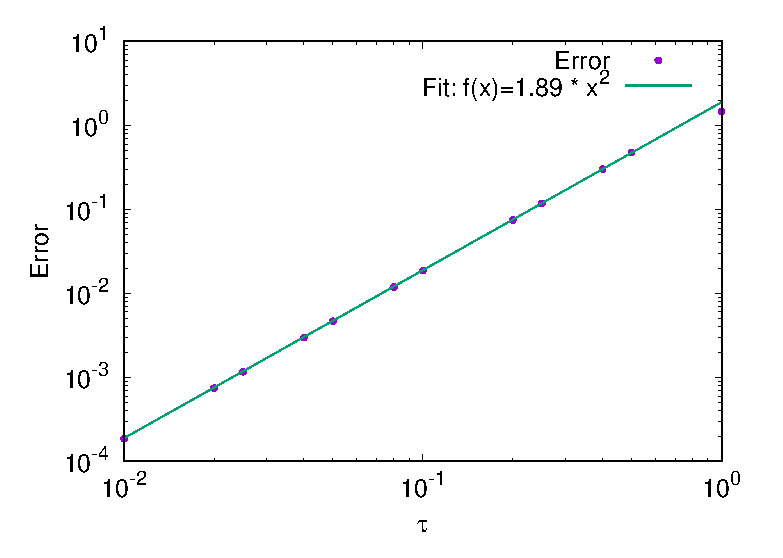
\includegraphics[scale=0.8]{Error.eps}
\caption{The error in the Suzuki-Trotter formula algorithm relative to the full diagonalization method. The involved error grows quadratically in $\tau$.}
\label{fig:o1}
\end{figure}
Since the dependence of the error on $\tau$ can be approximated to be linear in the log scale, as shown in Fig.~(\ref{fig:o1}), the simulation implementing TDSE can be trusted to be following the second order Suzuki-Trotter product formula algorithm.

\section{Selected Problems}
For a fixed $T_A$, the success probability is expected to decrease with decreasing $\Delta_{min}$, if the evolution of the state is close to adiabatic. In this section, three problems, with distinct minimum energy gaps and success probabilities are selected from the set of 12-spin problems, and their dynamics is studied.\\

As the first example, considered here is problem number 733, that has a high success probability. Figure~(\ref{fig:o2}), shows the energy spectrum for this problem. $\Delta_{min}$ is 0.4407 in this case. Also plotted in the figure are the energy expectation values for the instantaneous state obtained for the three annealing times.
\begin{figure}[H]
\centering 
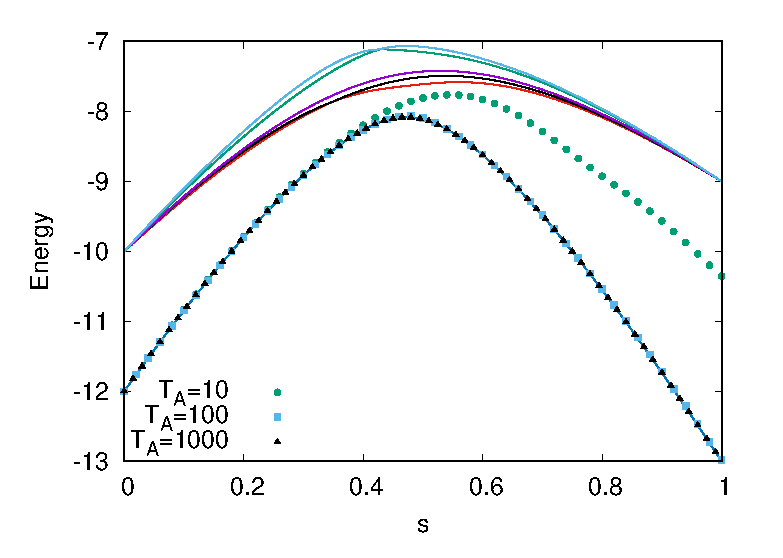
\includegraphics[scale=0.8]{733_s12_O.eps}
\caption{The energy spectrum for problem 733, with energy expectation values for the instantaneous state. $\Delta_{min}$ is found to be 0.4407.}
\label{fig:o2}
\end{figure}

As expected, the overlap of the final state with the ground state of the problem Hamiltonian increases on increasing the total annealing time in Fig.~(\ref{fig:o2}). Annealing times $T_A$=10, 100, 1000 yield $p$=0.3444, 0.9944, 0.9999 respectively.\\

Secondly, problem number 950, with a small success probability is chosen. Figure~(\ref{fig:o3}) shows the energy spectrum and the energy expectation values for the instantaneous state corresponding to three annealing times, for this problem. Annealing  times $T_A$=10, 100, 1000 yield $p$=0.0002, 0.0146, 0.1362 respectively. It should be noted, that the minimum gap for this problem is much smaller than in problem 733, and has a value of $\Delta_{min} = 0.0312$. This explains the decrease in success probability for the same annealing times.\\
\begin{figure}[H]
\centering 
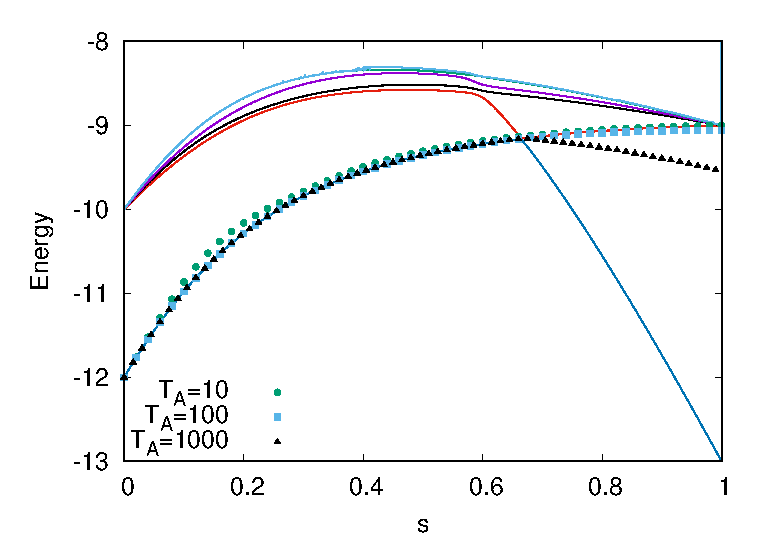
\includegraphics[scale=0.8]{950_s12_O.eps}
\caption{The energy spectrum for problem 950, with energy expectation values for the instantaneous state. $\Delta_{min}$ is found to be 0.0312.}
\label{fig:o3}
\end{figure}


As the final case, problem number 528, with an intermediate success probability is studied. For this case too, the energy spectrum and the energy expectation values for the instantaneous state, corresponding to the three annealing times were determined, as is shown in Fig.~(\ref{fig:o4}). Annealing times $T_A$=10, 100, 1000 yield $p$=0.1577, 0.5199, 0.9999 respectively. The value of the minimum gap is $\Delta=0.1573$ for this problem, which is intermediate to the above two cases. 
\begin{figure}[H]
\centering 
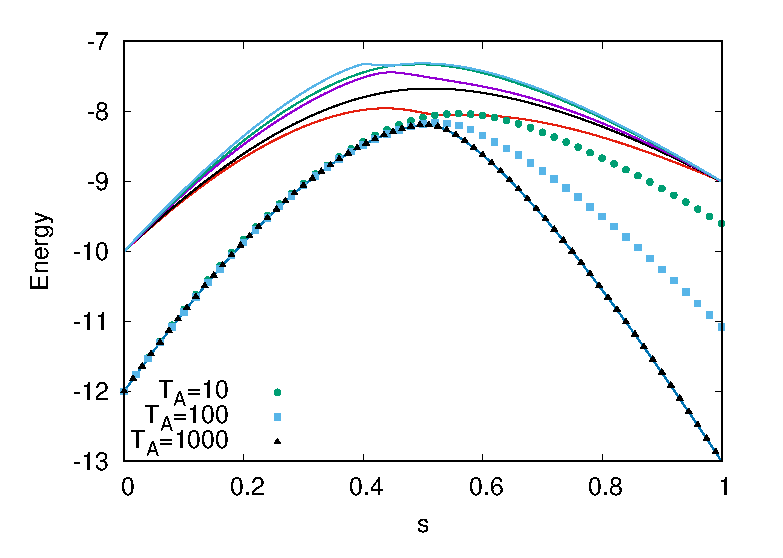
\includegraphics[scale=0.8]{528_s12_O.eps}
\caption{The energy spectrum for problem 528, with energy expectation values for the instantaneous state. $\Delta_{min}$ is found to be 0.1573.}
\label{fig:o4}
\end{figure}

\begin{comment}
The main feature of difference between the 12-spin and 8-spin problems is that the minimum energy gaps of the 8-spin problems were found to be larger than those of 12-spin problems. This can be understood with the help of Eq.~(\ref{eq:b10}), where the minimum gap is expected to close exponentially with increasing N. Even the gap corresponding to the case with smallest success probability in 8-spin problems (the smallest energy gap amongst 91 8-spin problems, $\Delta_{min}=0.4725$) is still larger than the the gap corresponding to the case with largest success probability in 12-spin problems (the largest energy gap amongst 1000 12-spin problems, $\Delta_{min}=0.4407$). Therefore, even an annealing time of $T_A=100$ yields a large success probability for almost all 8-spin cases. 
\end{comment}

Thus, for all the three problems, the state of the system deviates from the ground  state of the Hamiltonian when the annealing time is not long enough as required by the minimum energy gap of the problem for ensuring the evolution of the state to be strictly adiabatic. In all such cases, the system state deviates from the ground state only at the energy anti-crossing between the ground state and first excited state of the Hamiltonian. As the annealing time is increased, the part of the amplitude in the ground state that is shifted to the higher states gets smaller, thus increasing the success probability.

\section{The Bigger Picture}

\begin{figure}[H]
\centering 
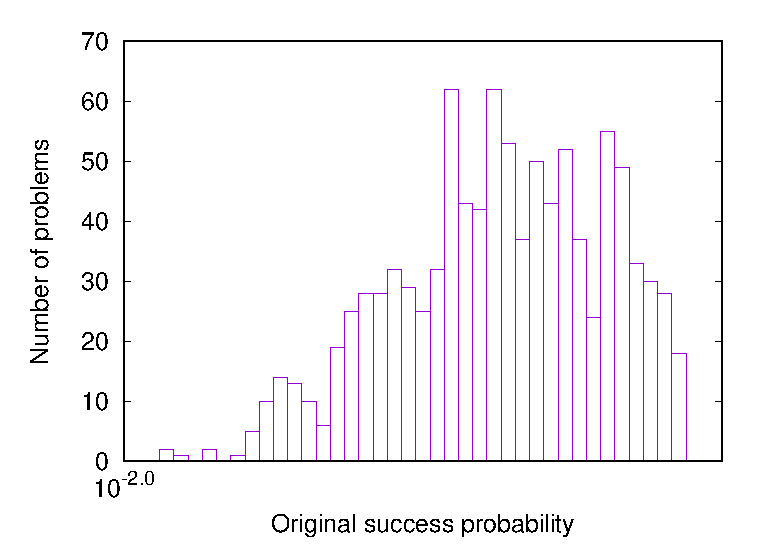
\includegraphics[scale=0.8]{O_s12_T100_g0.eps}
\caption{Histogram for the success probability of the Hamiltonians without any triggers ($g$=0) for 1000 12-spin problems for $T_A$=100.}
\label{fig:o8}
\end{figure}
We now focus on the entire set of the 12-spin problems to understand the performance of the quantum annealing algorithm with the original Hamiltonians (i.e. for $g$=0).\\
To obtain a rough estimate of the spread of the difficulty of the problems considered in this work, Fig.~(\ref{fig:o8}) shows a plot of the distribution of the success probabilities for all the problems in the set. The range of the success probability is from 0.014 for the most difficult cases, to 1 for the relatively easier cases. The mean success probability was found to be 0.208. 
Finally, Fig.~(\ref{fig:o10}) shows the success probability of all the 12-spin problems with the corresponding minimum energy gaps.
\begin{figure}[H]
\centering 
\includegraphics[scale=0.8]{Orig_GapVsSucc.eps}
\caption{Success probability versus minimum energy gaps for all the 12-spin problems for annealing times 10, 100 and 1000.}
\label{fig:o10}
\end{figure}
From Eq.~(\ref{eq:lz5}), the success probability should have the Landau-Zener dependence on the minimum energy gap between the ground and first excited state of the Hamiltonian, if the evolution of the state is close to adiabatic. Since different problems belonging to the set may have different values of $\Delta_{min}$, the success probability for each problem, plotted against the respective minimum energy gap for a fixed annealing time, can give an estimate of the fraction of problems undergoing nearly adiabatic evolution. The more is the scattering in the resulting curve, the larger is the fraction of problems involving non-adiabatic mechanisms during the evolution. It can therefore be noted in Fig.~(\ref{fig:o10}) that for $T_A$=10, the scattering is significantly larger than in the other two cases. It should additionally be observed that as the annealing time is increased, the success probability for a specific problem becomes systematically larger. This suggests that as the annealing time is increased, the evolution of the state keeps getting closer to adiabatic, as naively expected.


\end{document}